\documentclass[a4paper,11pt]{article}
\usepackage[utf8]{inputenc}
\usepackage{fullpage}
\usepackage{graphicx}
\usepackage{wrapfig}
\usepackage{caption}
\usepackage{subcaption}
\usepackage{appendix}
\usepackage{tcolorbox}
\tcbuselibrary{theorems}

\newtcbtheorem[number within=section]{theo}{}%
{colback=green!5,colframe=green!35!black,fonttitle=\bfseries}{th}

\title{% 
	4F12: Computer vision \\
	\vspace{10pt}
	\small Summarized from I. Budvytis \& S. Albanie lectures, Michaelmas 2021}
\author{\small Oussama Chaib}
\date{\small October 2021}

\begin{document}
	\maketitle
		\tableofcontents
		\pagebreak
\section{Introduction}
\subsection{Preamble}
Threefold goal to the course:
\begin{enumerate}
	\item Define computer vision
	\item Motivation to study computer vision
	\item Ways computer vision problems can be formulated so they can be addressed by computer algorithms.
\end{enumerate}
\subsection{What is computer vision?}
First questions include the definition of computer vision and motivation to study it. Vision is our most powerful sense (more than 50\% of the brain's cortex is devoted to vision and related tasks). Discovering from images what is in the scene and so on.
\vspace{5pt}
\\
\textbf{Definition --} Computer vision is a collection of algorithms which capture process and interpret images of a scene to extract useful information about the scene.
\vspace{5pt}
\\
\textit{Examples --} Reconstructing objects from a scene (3D shape), discovery of location of image, semantic segmentation of the image (each pixel assigned a label, i.e: person, car, building etc.)\vspace{5pt}\\
All these examples correspond to three different tasks in computer vision (also known as \textbf{3 R's}):
\begin{enumerate}
	\item \textbf{Representation/reconstruction} (Geometrical framework): Recover 3D shape.
	\begin{itemize}
		\item Image acquisition (camera): Get points and depth of each pixel or mesh.
		\item Get features: Since analyzing all pixels is computationally intensive, and in order to simplify the image (i.e: edges, corners, blobs...)
	\end{itemize}
	\item \textbf{Registration} (Statistical framework): Compute position or pose.
	\begin{itemize}
		\item Register the position of the camera with respect to the coordinate system.
		\item Applications: VR, VAR indoors (i.e: IKEA app that allows users to view projected objects as if they are in the environment).
	\end{itemize}
	\item \textbf{Recognition} (Machine learning and data): Identify objects.
	\begin{itemize}
		\item Deep learning for computer vision.
		\item Applications: facial recognition, object recognition (autonomous driving, labeling objects in surrounding environment for visually impaired people, app that captions drawings on board).
		\item These techniques are powerful but they may be learning features that are "too simple" (knowing the theory is important).
	\end{itemize}
\end{enumerate}
Computer vision isn't exactly the same as image processing and pattern recognition. Image processing: converting the input to output (more desirable image). Pattern recognition: a certain class of computer vision, require examples. \vspace{5pt}\\
\textbf{Why study computer vision?} Curiosity, lots of applications of vision in real life.\\
\textit{Some examples:} autonomous vehicles, automation, human-computer interaction, augmented reality, security, medical imaging, 3D modelling and measurements.\vspace{5pt}\\
\textbf{Starting from biology --} The eye is, in many ways, an optical camera, while the brain would be similar to a collection of computer algorithms (complex human neural network where each part of the brain is in charge of a certain thing). An electric impulse is created at the retina, sent to the brain neural network, then a signal is sent to the spinal cord/body so the body can react.\vspace{5pt}\\
\textbf{Why don't we directly copy the brain?} It's quite complex, we don't know everything about it, might be hard to replicate and costly as well. It took a certain level of constraints for the brain to evolve to what it is today. Direct copying of the brain may also not be very revealing.\\
\textit{Solution:} Instead of directly copying the brain, we could get inspired by it! Deep learning methods for example.\vspace{5pt}\\
\textbf{Building a computer vision algorithm --} Several parts:
\begin{itemize}
	\item \textbf{Camera :} Convert light to electric signals, convert the encoded signal into a 3D array (with different channels for colors for example, i.e: RGB). Image formation is a \textbf{many-to-one} mapping. Inverse imaging is quite challenging since the images only tell us along which ray a feature lies and not how far along the ray (called image depth).\\
	% Insert image planes fig
	These ambiguities are typically used in art to create optical illusions (i.e. Ames room with slanted wall).\\
	% Insert 2 person photos Wall slanted, 2nd person standing much further than the 2nd person (Ames room)
	Images are unstructured 2D arrays. Before using them, they should be processed to reduce the amount of information so it is directly relevant to solving the problem (these are called image features, i.e: edges, blobs...).\\
	\textbf{Image feature --} Piece of info about a certain region of an image that contains certain desirable properties. We decide which features to extract based on what problem we would like to solve.\\
	How do we reduce ambiguities? Drawing a set of constraints. i.e: one solution is to use multiple images instead of one. We can introduce assumptions about the world in the imaging scene (i.e: a face contains two eyes and a nose and a mouth). Deep learning is interesting in that sense because it will help determine those assumptions/constraints from labeled and unlabeled data.
	\item \textbf{Feature extraction:} What do they look like? How can they be obtained? Example: edges: discontinuities in images (filtering by smoothing kernel, then looking for largest gradient magnitudes), corners: areas in image with large changes in local curvature.
	\item \textbf{Perspective projection:} Establishing a camera model. Accounts for the position of the camera, perspective projection, position of CCD array on image plane. How 3D coordinates of a point in a scene is matched to a pixel coordinate in an image? All of this is studied within the framework of \textbf{perspective geometry}. Lines from planes parallel to image plan all intersect in vanishing points.
\end{itemize}

Most algorithms tasked with extraction of 3D information from images make very few assumptions about the scene or 3D image. Some types:
\begin{itemize}
	\item \underline{\textbf{Shape from texture:}} Simple assumptions: either homogenous (brick wall) or isotropic textures. Can infer orientation of surfaces from analyzing how the texture statistics vary over the image.
	\item \underline{\textbf{Stereo vision:}} Assuming the scene is viewed from two cameras. The constraints are in this case relaxed. Features should be matched using two different images (known as \textbf{correspondance problem}) as long as the two cameras are calibrated. Otherwise, we can only recover 3D features using \textbf{projective ambiguity} (to be seen later). The 3D structure can be reconstructed to scale (to be seen later too).
	\item \underline{\textbf{Structure from motion:}} Similar to stereo vision, but instead of using two pictures we allow the camera to move and collect several images/collect a sequence from different viewpoints. 
	\item \textbf{Shape from contour: } Instead of tracking 2D points (structure from motion), apparent contours of the the image are tracked. Not covered in this class.
	\item \textbf{Shape from shading:} Unlike the two previous methods, doesn't require camera motion. Uses knowledge from how light reflects in scenes/objects. Also not covered.
\end{itemize}

\subsection{Geometrical and statistical frameworks}
Algorithms introduced in previous section belong to a certain \textbf{geometrical framework}. Three key steps in geometric frameworks:
\begin{enumerate}
	\item Reduce the information content of an object by extracting useful features (edges, corners, blobs).
	\item Model the imaging process (usually using perspective projection) and express using projective transformations). 
	\item Invert the tranformation using as many images and constraints as possible to extract 3D structure and motion.
\end{enumerate}
Not all problems can be studied using geometrical framework (example: determining the family of cats in an image). In this case, \textbf{statistical frameworks} perform better. They often involve some learning process from a collective set of images with the ability to estimate the confidence of your model. \\
We will look closely at one type of deep learning architecture:  \textbf{convoluted neural networks (CNN)}. They have multiple layers of feature reponses which are obtained by filtering/convolution and non-linear activation functions. The weights of each filter are learned by training the algorithm (millions or billions of parameters!). They are very effective in many computer vision tasks and need large data sample. 
	
\section{Image structure}
\subsection{Representing images as intensities:}
How are images stored on a computer? The simplest way to store a monochrome (grayscale) image is a matrix of intensity values $I(x,y)$. We use 256 discrete values (8-bit, $2^8$) to represent intensities (0: black, 255: white). In addition to intensities, we also use resolutions to represent the size of matrices. Color images can be represented by stacking matrices of RGB channels (primary colors of light).
\subsection{Challenges}
\begin{itemize}
	\item \textbf{Nuisance factor:} The intensity of a point $P(x,y)$ is affected by many \textbf{geometric} and \textbf{photometric} "nuisance factors" such as:
	\begin{itemize}
		\item Position and orientation of camera.
		\item Geometry of the scene (3D shapes and layout).
		\item Nature and distribution of light sources.
		\item Reflectance properties of surfaces (Lambertian, albedo/reflection of incoming radition 0 (black body), 1 (white)).
		\item Properties of camera lens and sensor array.
	\end{itemize}

	\item \textbf{Data reduction:} A current challenge for modern computers. To give a scale, raw image data from a GoPro is $O(10\, Gbits/s)$ at 60 fps. For an iSight CCD camera, it is $O(100\, Mbits/s)$ at 30 fps. Both are impractical in our case as the images we would like to use should be of $O(100\, Kbits/s)$. To reduce the order we can:
	\begin{enumerate}
		\item Capture raw image data.
		\item Extract salient features: Should be as generic as possible, we can discard the original image and perform all our analyses on the generic features, while preserving the useful information in images (albedo changes, 2D shape of objects in the scene).
		\item Interpret.
	\end{enumerate}
\end{itemize}
\subsection{Computer vision as a hierarchical process}
Multiple theories of the human vision hierarchy in neuroscience literature. Usually starts off with a raw image that is sent to the \textbf{vision system}. A high-level question is asked (i.e: Is this animal dangerous?) and an action is triggered depending on the answer to that question. Similarly, computer vision takes raw images as perceived intensities then performs a primal sketch (data reduction: blobs, edges, zero-crossings, groups), a 2.5D sketch (local surface, orientation, distance from viewer, depth discontinuities), then a 3D model representation to address the high-level question. 
\subsection{Structure of an image}
Example of an image with a person. The featureless region has a smooth variation of intensities (approximately constant intensity pixel values in the region). Edges reveal intensity discontinuities in \textbf{one} direction (cliff-life structure), while corners reveal an intensity discontinuity in \textbf{two} directions (a bit hard to interpret from intensity pixel plot). \\
\textbf-- {Edges and corners are practically invariant to lighting --} (intensity discontinuities are likely to remain prominent whatever the lighting conditions) Very desirable since lighting conditions can be a nuisance factor.
\subsection{Edge detection}
\subsubsection{How to perform 1D Edge detection?}
\begin{enumerate}
	\item \textbf{Smoothing} the original raw signal $I(x)$ to reduce or suppress noise. \\
	\underline{\textit{Solution:}} Gaussian filter -- a low pass filter that suppresses high-frequency noise.\\
	We first convolve the signal $I(x,y)$ with a Gaussian kernel $g_\sigma (x)$ of standard deviation $\sigma$ to produce a smooth signal:
	\begin{center}
		\fbox{$g_\sigma (x)=\frac{1}{\sigma \sqrt{2\pi}} e^{-\frac{x^2}{2\sigma ^2}}$}
		\vspace{5pt}\\
		\fbox{$s(x)=I(x)*g_\sigma (x) = \int_{-\infty}^{+\infty}g_\sigma(u) I(x-u)du =  \int_{-\infty}^{+\infty}g_\sigma(x-u) I(u)du$}
	\end{center}
	\item Compute \textbf{derivative} of smoothed function $s'(x)$.
	\item Find \textbf{maxima} and \textbf{minima} of $s'(x)$.
	\item Use \textbf{thresholding} on the magnitude of the extrema to mark the edges.
	\begin{figure}[h]
		\centering
		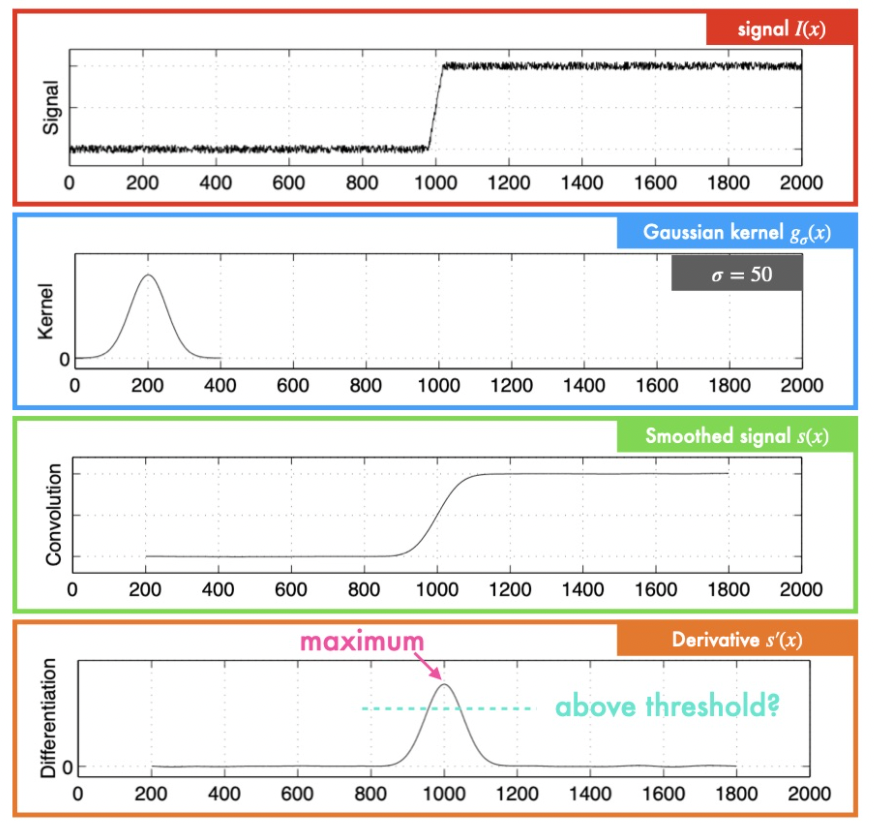
\includegraphics[width=0.8\linewidth]{figures/1Dedge.png}
	\end{figure}
\end{enumerate}
\subsubsection{Computational tricks for faster edge detection!}
\begin{enumerate}
	\item \textbf{Derivative of convolution:} Instead of smoothing and \textit{then} derivating the smooth function (in this case, we make use of two convolutions: one for the smoothing and another for the derivate, we'll see the latter one later in the course), we can combine both steps using the \textbf{derivative theorem of convolution} (\emph{note that convolution is commutative}):
	\begin{center}
	\fbox{$s'(x)=\frac{d}{dx}(I(x)*g_\sigma(x))=g'_\sigma(x)*I(x)$}
\end{center}
	\item \textbf{Second derivative $s''(x)$:} Instead of finding the minimum and maximum of $s'(x)$, we can try to find the zero-crossings of $s''(x)$. These zero-crossings mark possible edges.
\end{enumerate}
\subsubsection{1D Edge detection scale}
The question of which $\sigma$ value to use is relevant and depends on the specific features we would like to emphasize. Smaller values of $\sigma$ bring out all the edges, modest values bring out edges at a fine scale, while larger values of sigma will one focus on the larger coarse/rough scales. \\
\emph{Note:} Fine scale edge detection is (as one would imagine) more sensitive to noise. 
\subsubsection{Generalizing to 2D edge detection}
\textbf{-- Basic approach: Canny edge detection} (directional edge detection, trick 1)
\begin{enumerate}
	\item \textbf{Smoothing} using a 2D Gaussian kernel $G_\sigma (x,y)$
		\begin{center}
		\fbox{$G_\sigma(x,y)=g_\sigma (x).g_\sigma (y)=\frac{1}{\sigma^2 2\pi} e^{-\frac{x^2+y^2}{2\sigma ^2}}$}
		\vspace{5pt}\\
		\fbox{$S(x,y)=G_\sigma (x,y)*I(x,y)=\int_{-\infty}^{+\infty}\int_{-\infty}^{+\infty} G_\sigma (u,v) I(x-u,y-v) du dv$}
	\end{center}
	\item \textbf{Derivation/Gradients:} We then compute the gradient of the smooth function using the derivative theorem of convolution:
	\begin{center}
		\fbox{$\nabla S = [\frac{\partial G_\sigma (x,y)}{\partial x},\frac{\partial G_\sigma (x,y)}{\partial y}]$}
	\end{center}
	\item \textbf{Non-maxima suppression:} Edge elements (edgels) are placed in positions where $|\nabla S|$ is greater than local values of $|\nabla S|$ in the correct direction ($|\nabla S_x|$, $|\nabla S_y|$).\\
	\emph{(en gros, on calcule les gradients max par rapport aux gradients dans leur voisinage proche et dans la bonne direction)}
	\item \textbf{Thresholding}.
\end{enumerate}
\textbf{-- Faster approach: Marr-Hildreth edge detection --} (isotropic edge detection, trick 2)
Makes use of the second derivative $S''(x,y)$:
\begin{center}
	\fbox{$S''(x,y)=\nabla^2 G_\sigma(x,y)*I(x,y)$}
\end{center}

\subsubsection{Implementation of 2D convolution and differentation}
\textbf{-- 2D Convolution}\\
In reality, we don't use infinite integrals because the computational power is large. Instead, we use truncated sums:
\[S(x,y)=\sum_{u=-n}^{n}\sum_{v=-n}^{n} G_\sigma(u,v) I(x-u,y-v)\]
The largest mass of the Gaussian kernel is usually between $-3 \sigma$ and $+3 \sigma$. As a rule of thumb, we discard samples less than $1/1000$ of the peak value.
We use a $2n+1$ size kernel ($-n$ to $+n$). The higher the value of $\sigma$, the higher the value of $2n+1$.
\vspace{5pt}\\
\textbf{Computational trick --} Decomposing a 2D convolution to a set of two 1D convolutions:
\begin{center}
	\fbox{$S(x,y)=G_\sigma (x,y)*I(x,y)=g_\sigma(x)*(g_\sigma (y)*I(x,y))$}
\end{center}
\textbf{Why is differentiation also a convolution?}\\
The differentiation of the smooth image is also done by discrete convolution. The first-order spatial derivative of $S(x,y)$ with respect to x is, in this case, approximated by a discrete finite difference using a Taylor series expansion of $S(x,y)$:
\vspace{5pt}\\
\emph{Reminder:} Taylor series expansion:
\[f(u+h)=f(u)+h.f'(u)+\frac{h^2}{2!}.f''(u)+\frac{h^3}{3!}.f^{3}(u)+...\]
With $u=x-1$ and $h=2$, we get:
\[S(x+1,y)=S(x-1,y)+2.\frac{\partial S}{\partial x}\]
The finite difference is then defined as:
\begin{center}
	\fbox{$\frac{\partial S}{\partial x}=\frac{S(x+1,y)-S(x-1,y)}{2}$}
\end{center}
Example:
\begin{figure}[h]
	\centering
	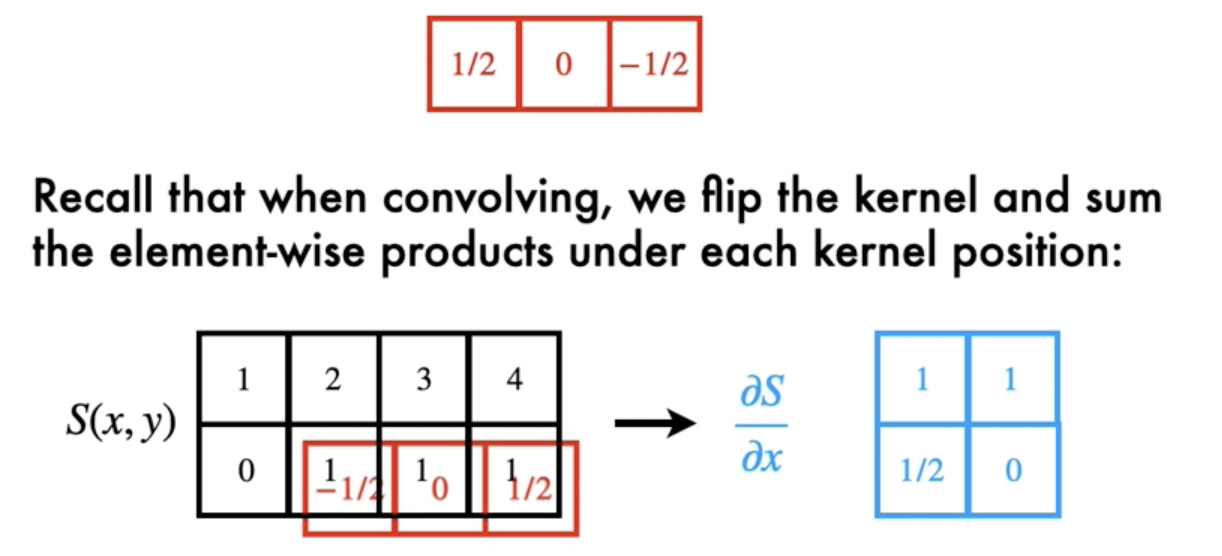
\includegraphics[width=.6\linewidth]{figures/diff.png}
\end{figure}
\end{document}






